
\section{Ejercicio 2}

\subsection{Problema: Algo Rush}
El Pabell\'on 0+infinito acaba de reabrir sus puertas con la novedad de que ahora tiene P portales que
son bidireccionales; asimismo, los paraca\'idas fueron eliminados por considerarse inseguros. Cada piso del renovado pabell\'on consta de un pasillo de L metros de longitud, y cada portal permite viajar entre
posiciones espec\'ficas de los pasillos de dos pisos. M\'as concretamente, cada portal puede describirse por
medio de cuatro enteros no negativos A, DA, B y DB, los cuales indican que el portal comunica el
piso A, a DA metros del comienzo del pasillo de ese piso, con el piso B, a DB metros del comienzo
del pasillo de ese piso. Los alumnos, acostrumbrados a los portales que s\'olo permitan subir, est\'an un
poco confundidos al poder utilizar un mismo portal tanto para subir como para bajar entre dos pisos, o
incluso para moverse entre posiciones diferentes dentro del pasillo de un mismo piso. Todos los alumnos
de Algoritmos III quieren llegar primero a la clase, que es en un aula que est\'a al final del piso N (el m\'as
alto del pabell\'on). Dise\~nar un algoritmo de complejidad O(NL + P) para calcular la m\'inima cantidad
de segundos que se necesitan para llegar del comienzo del pasillo del piso 0 al final del pasillo del piso
N, suponiendo que recorrer un metro requiere 1 segundo, y utilizar cualquier portal requiere 2 segundos
(en cualquiera de las dos direcciones posibles). Se asegura que en toda instancia del problema es posible
realizar el recorrido deseado, y que no hay m\'as de un portal que comunique las mismas posiciones del
mismo par de pisos. No obstante, puede haber m\'as de un portal que comunique el mismo par de pisos,
y portales que comuniquen posiciones diferentes dentro del pasillo de un mismo piso.\\

Este problema esta planeado de una manera parecida al anterior tendiendo como diferencia principal que ahora los portales son bidireccionales y que el primero quiere maximizar la cantidad de portales usados y este desea minimizar el tiempo para llegar desde el principio hasta el final. La medida del tiempo, com bien dice el enunciado, depende de la cantidad de portales que utilicemos y de la cantidad de metros que caminemos. Cada portal que utilicemos nos tomara 2 segundos y cada metro que camienmos nos aumentara 1 segundo.

\pagebreak
\subsubsection{Explicacion del Problema}
    El problema consiste en minimizar la cantidad de tiempo que se tarda en llegar desde el inicio de la planta baja hasta el final del ultimo piso. Esto puede ser representado por un grafo donde los nodos representan los portales (el inicio de la planata baja y el final del ultimo piso tambien) y los ejes los metros (o segundos) entre un portal y otro, observar que para este caso los ejes son bidireccionales ya que se puede ir y volver por los portales. Si el eje representa la conexion entre dos portales que esten conectados su peso sera 2 y, de no estar conectados y ser adyacentes en el mismo piso, equivaldra a la distancia que exista entre ambos.
    
    \begin{figure}
    \centering
    
    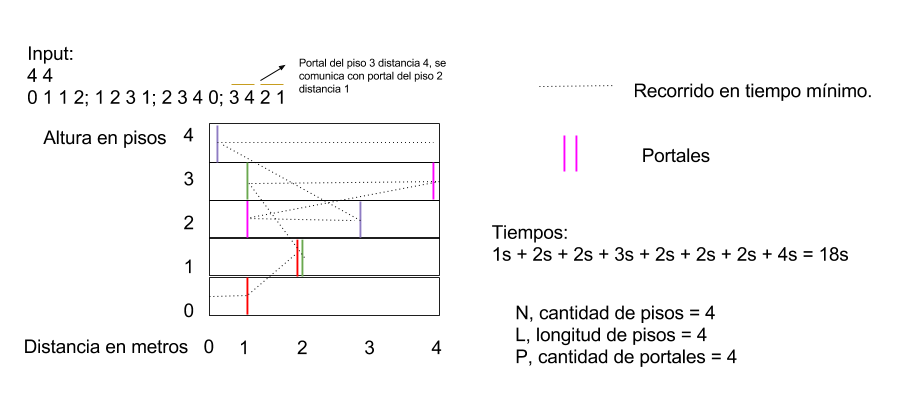
\includegraphics[scale=0.5]{imagenes/dibujito2.png}
    \caption{representacion de pisos y portales y su solucion}
    \label{fig:my_label}
    
    \tikzset{main node/.style={circle,fill=white!20,draw,minimum size=0.5cm,inner sep=0pt},}
\begin{tikzpicture}
    %\begin{scope}[xshift=4cm]
    \node[main node] (1) {1};
    \node[main node] (2) [right = 0.7cm  of 1] {2};
    \node[main node] (3) [above right = 0.7cm and 0.5cm of 2] {3};
    \node[main node] (4) [right = 0.1cm of 3] {4};
    \node[main node] (5) [above left = 0.7cm and 0.5cm of 3] {5};
    \node[main node] (6) [right = 1.5cm of 5] {6};
    \node[main node] (7) [above = 0.7cm of 5] {7};
    \node[main node] (8) [right = 2cm of 7] {8};
    \node[main node] (9) [above left = 0.7cm and 0.5 of 7]{9};
    \node[main node] (10) [right = 3.0cm of 9] {10};


    \path[draw,thick]
    (1) edge node {$1$} (2)
    (2) edge node {$2$} (3)
    (4) edge node {$2$} (7)
    (6) edge node {$2$} (9)
    (8) edge node {$2$} (5)
    (2) edge node {$2$} (3)
    (3) edge node {$0$} (4)
    (5) edge node {$2$} (6)
    (7) edge node {$3$} (8)
    (9) edge node {$4$} (10)
    ;
    %\end{scope}
\end{tikzpicture}

    \caption{representacion en un grafo del ejemplo anterior}
    \end{figure}
    
    Para solucionar el problema se cuenta con una cota m\'axima de $O(N*L + P)$ con N cantidad de pisos, L longitud de cada piso y P cantidad total de portales.
    
\subsubsection{Explicacion del Desarrollo}
    Se cuenta con un grafo con pesos distintos en sus ejes, sobre el mismo habra una cantidad total de $P + 2$ nodos (cantidad de portales mas nodo inicial y final). 
    A continuacion se analizara una modificacion del grafo, para esto definimos: \\

    Sea $G$ un grafo conexo con pesos posisitivos en sus ejes y $v$,$w$ cualquier par de vertices adyacentes de $G$, llamamos $G'$ al grafo donde el peso $p$ en el eje que conecta v con w es reemplazado por $p - 1$ nodos intermedios (de peso 1 en sus ejes) entre v y w, siendo asi $G'$ un grafo con peso uniforme en sus ejes. \\

    \begin{center}
        \tikzset{main node/.style={circle,fill=white!20,draw,minimum size=1cm,inner sep=0pt},}
\begin{tikzpicture}
    \node[main node] (1) {$A$};
    \node[main node] (2) [right = 1.5cm of 1]  {$B$};

    \path[draw,thick]
    (1) edge node {$2$} (2)
    ;
    %%
    \begin{scope}[xshift=4cm]
    \node[main node] (1) {$A$};
    \node[main node] (3) [right = 1.5cm  of 1] {};
    \node[main node] (2) [right = 1.5cm  of 3] {$B$};

    \path[draw,thick]
    (1) edge node {$1$} (3)
    (3) edge node {$1$} (2)
    ;
    \end{scope}
\end{tikzpicture}
\\Ejemplo nodos fantasma para un eje de peso 2
    \end{center}
    
    El nuevo grafo $G'$ colocara nodos intermedios entre los nodos de $G$, como puede haber un nodo en cada punta de los pisos (metro 0 y L) se pueden generar hasta $L-2$ nodos intermedios por piso, aplicandolo a todos los pisos queda $N * (L - 2)$ nodos totales, falta tener en cuenta las conexiones entre portales a las cuales se les agrega un nodo a cada una con lo que quedaria $N * (L - 2) + P$ con lo que puede ser acotado por $N*L + P$ nodos totales \endl\\
    
    Por lo visto en clase el algoritmo $BSF$ tiene complejidad lineal sobre la cantidad de nodos del grafo y puede encontrar el camino minimo entre $2$ nodos si los pesos son constantes en sus ejes, si trabajamos con $G'$ podemos ver que cumple con las condiciones que pide BFS y su complejidad sera $O($cantidad de nodos de $G') = O(N*L + P)$ que es la complejidad pedida.
    
    \begin{figure}
    \centering
    \tikzset{main node/.style={circle,fill=white!20,draw,minimum size=0.75cm,inner sep=0pt},}
\begin{tikzpicture}
    
        \node[main node] (1) {0};
        \node[main node] (2) [right = 3.5cm of 1]  {};
        \node[main node] (3) [above = 1.5cm of 1]  {};
        \node[main node] (4) [right = 1.9cm of 3]  {};
        
        \node[main node] (5) [above = 3.5cm of 2]  {};
        \node[main node] (6) [left  = 1.8cm of 5]  {};
    
        \path[draw,thick]
        (1) edge node {} (2)
        (2) edge node {} (3)
        (2) edge node {} (5)
        (3) edge node {} (4)
        (3) edge node {} (6)
        (4) edge node {} (6)
        (5) edge node {} (6)
        (5) edge node {} (1)
        ;
        
        \begin{scope}[xshift=6cm]
            \node[main node] (1) {0};
            \node[main node] (2) [right = 3.5cm of 1]  {1};
            \node[main node] (3) [above = 1.5cm of 1]  {};
            \node[main node] (4) [right = 1.9cm of 3]  {};
            
            \node[main node] (5) [above = 3.5cm of 2]  {};
            \node[main node] (6) [left  = 1.8cm of 5]  {};
        
            \path[draw,thick]
            (1) edge[red] node {} (2)
            (2) edge node {} (3)
            (2) edge node {} (5)
            (3) edge node {} (4)
            (3) edge node {} (6)
            (4) edge node {} (6)
            (5) edge node {} (6)
            (5) edge node {} (1)
            ;
        \end{scope}
        
        \begin{scope}[yshift=-6cm]
            \node[main node] (1) {0};
            \node[main node] (2) [right = 3.5cm of 1]  {1};
            \node[main node] (3) [above = 1.5cm of 1]  {};
            \node[main node] (4) [right = 1.9cm of 3]  {};
            
            \node[main node] (5) [above = 3.5cm of 2]  {1};
            \node[main node] (6) [left  = 1.8cm of 5]  {};
        
            \path[draw,thick]
            (1) edge node {} (2)
            (2) edge node {} (3)
            (2) edge node {} (5)
            (3) edge node {} (4)
            (3) edge node {} (6)
            (4) edge node {} (6)
            (5) edge node {} (6)
            (5) edge[red] node {} (1)
            ;
        \end{scope}
        
        \begin{scope}[yshift=-6cm,xshift=6cm]
            \node[main node] (1) {0};
            \node[main node] (2) [right = 3.5cm of 1]  {1};
            \node[main node] (3) [above = 1.5cm of 1]  {2};
            \node[main node] (4) [right = 1.9cm of 3]  {};
            
            \node[main node] (5) [above = 3.5cm of 2]  {1};
            \node[main node] (6) [left  = 1.8cm of 5]  {};
        
            \path[draw,thick]
            (1) edge node {} (2)
            (2) edge[red] node {} (3)
            (2) edge node {} (5)
            (3) edge node {} (4)
            (3) edge node {} (6)
            (4) edge node {} (6)
            (5) edge node {} (6)
            (5) edge node {} (1)
            ;
        \end{scope}
        
        \begin{scope}[yshift=-12cm]
            \node[main node] (1) {0};
            \node[main node] (2) [right = 3.5cm of 1]  {1};
            \node[main node] (3) [above = 1.5cm of 1]  {2};
            \node[main node] (4) [right = 1.9cm of 3]  {};
            
            \node[main node] (5) [above = 3.5cm of 2]  {1};
            \node[main node] (6) [left  = 1.8cm of 5]  {2};
        
            \path[draw,thick]
            (1) edge node {} (2)
            (2) edge node {} (3)
            (2) edge node {} (5)
            (3) edge node {} (4)
            (3) edge node {} (6)
            (4) edge node {} (6)
            (5) edge[red] node {} (6)
            (5) edge node {} (1)
            ;
        \end{scope}
        
        \begin{scope}[yshift=-12cm, xshift=6cm]
            \node[main node] (1) {0};
            \node[main node] (2) [right = 3.5cm of 1]  {1};
            \node[main node] (3) [above = 1.5cm of 1]  {2};
            \node[main node] (4) [right = 1.9cm of 3]  {3};
            
            \node[main node] (5) [above = 3.5cm of 2]  {1};
            \node[main node] (6) [left  = 1.8cm of 5]  {2};
        
            \path[draw,thick]
            (1) edge node {} (2)
            (2) edge node {} (3)
            (2) edge node {} (5)
            (3) edge node {} (4)
            (3) edge node {} (6)
            (4) edge[red] node {} (6)
            (5) edge node {} (6)
            (5) edge node {} (1)
            ;
        \end{scope}
\end{tikzpicture}
    \caption{Algoritmo BFS}
    \label{fig:my_label}
    \end{figure}
    
    \pagebreak
    %Veamos un ejemplo: sean A, B dos vertices adyacentes $\in G$ cuyo eje tiene peso 5, por la definicion anterior existe un camino en $G'$ entre A y B donde todos los ejes tienen peso 1 y el peso del camino equivale al peso del eje entre A y B en $G$.
    %De esta manera s\'olo habra ejes de peso 1, por lo se puede utilizar el algoritmo BFS.\\  \¿Por qu\'e funciona este algoritmo en la nueva representaci\'on? Al estar a distancia 1 del primer nodo agregado, se expandera hacia sus vecinos, (observar que agrega solo 1 al peso total de los caminos que recorre), los cuales pueden ser nodos fantasma agregados o nodos en $G$, luego por cada vecino se expandera nuevamente(tambien agregando 1 al peso total) y asi sucesivamente. De esta manera en el momento en que el algoritmo encuentre el nodo buscado por primera vez, como cualquier proxima iteracion hara que todos los caminos tengan peso al menos 1 mas que el actual, ese sera el de menor peso.\endl\\

\subsection{Justificaci\'on y Complejidad}
La complejidad esta dada por: \endl
A) Transformar el grafo\endl
\begin{lstlisting}
Grafo2(List<Portal<Baldoza>> portales, int pisos, int mts) {
		this.mts = mts;//O(1)
		pisosUsados = new Boolean[pisos + 1];//O(pisos+1)
		FOR i desde 0 hasta pisosUsados.length
			pisosUsados[i] = false;//O(1)
		ENDFOR//O(pisos + 1)
		nodos = new Nodo[pisos+1][mts+1];//O(1)
		nodosFantasmas = new LinkedList<Nodo>();//O(1)
		idVertices = 0;//O(1)
	
		FOR portales AS portal
			Baldoza b1 = (Baldoza) portal.getDesde();//O(1)
			Baldoza b2 = (Baldoza) portal.getHasta();//O(1)
			connect(b1,b2);//O(CONNECT(B1,B2))
		}//O(ITERACIONES*CONNECTBALDOZAS)
		ENDFORECH
END
\end{lstlisting}


Por ahora nuestra complejidad es de $\BigO(N + P * connect(Baldoza, Baldoza))$ , por lo tanto debemos analizar la funci\'on connect para poder determinar nuestra complejidad.

Veamosla a continuaci\'on:

\begin{lstlisting}	
connect(Baldoza b1, Baldoza b2) 
	checkFloor(b1);//O(CHECKFLOOR(B1))
	checkFloor(b2);//O(CHECKFLOOR(B2))

	addNodo("FANTASMA", nodoFantasma) 
	connectNodos(b1.getPiso() + "," + b1.getMetros() , "FANTASMA,"+ nodoFantasma)
	connectNodos("FANTASMA,"+ nodoFantasma , b2.getPiso() + "," + b2.getMetros())
	nodoFantasma++	
END
\end{lstlisting}

Por lo tanto podemos acotar esta funci\'on por $\BigO(N + 2 * checkfloor() + 2 * connectNodos())$ en la cual nos falta determinar la complejidad de las 2 funciones.
Nuestra complejidad nos quedaria : $\BigO(N + N * (2 * checkfloor() + 2 * connectNodos()))$

Ahora veamos una de las dos funci\'ones que nos quedan, connectNodos, para la cual vamos a necesitar el analisis conjunto con la funci\'on addVecino la cual nos provee nuestra clase NODO, que lo que permite es agregar un nuevo vecino:

\pagebreak

\begin{lstlisting}
connectNodos(String string, String string2)
	Nodo a = getNodo(string);//O(1)
	Nodo b = getNodo(string2);//O(1)
	IF ! a.getVecinos().contains(b) //O(P)
           a.addVecino(b);//O(ADDVECINO(A))
	ENDIF
	IF ! b.getVecinos().contains(a)//O(P)
            b.addVecino(a);//O(ADDVECINO(B))
	ENDIF
END
\end{lstlisting}

\begin{lstlisting}
addVecino(Nodo vecino) 
	vecinos.add(vecino);   //O(1)
\end{lstlisting}

Podemos acotar la funci\'on connectNodos en $\BigO(P)$, ya que todas las operaci\'ones cuestan $\BigO(1)$, excepto el contains , y esto surge de una buena elecci\'on de las estructuras.

En este estado del analisis podemos afirmar que nuestra complejidad temporal es de : $\BigO(N + N * (2 * checkfloor()))$


\begin{lstlisting}
checkFloor(Baldoza b2){
	IF !pisosUsados[b2.getPiso()]
	    pisosUsados[b2.getPiso()] = true;//O(1)
		FOR j desde 0 hasta mts + 1
			addNodo(b2.getPiso(), j);  //O(1)
		ENDFOR
		FOR j desde 0 hasta mts 
			int k = j + 1;//O(1)
			connect(b2.getPiso()+","+j, b2.getPiso()+","+k); //O(1)
		ENDFOR
	ENDIF
END
\end{lstlisting}
Esta funci\'on es la encargada de generar todos los portales fantasmas por cada piso, una vez que se ingresa un nuevo portal, si y solo si no ingreso un portal del mismo piso anteriormente. Por lo tanto vamos a ver la cota cuando este piso no es creado es de $\BigO(1)$.
Podemos que ver que son todas operaci\'ones que cuestan $\BigO(1)$, y vemos que hay dos For's que iteran para generar los nodos, estos hacen L+1 y L iteraci\'ones, por lo tanto la complejidad es : $\BigO(L+1 + L)$ , lo que nos queda, $\BigO(L)$. Para llegar a esto debimos ver que la complejidad de addNodo era $\BigO(1)$, la cual se puede extraer del siguiente analisis:

Para esta funci\'on hicimos un uso de una funcionalidad de java, que es la sobrecarga de metodos, la cual permite tener varios metodos con el mismo nombre, pero se utiliza la correspondiente a la aridad de los parametros. Por lo tanto tenemos 2 metodos que se llaman $"$addNodo$"$.

\pagebreak

\begin{lstlisting}
addNodo(int piso, int mts)
    IF nodos[piso][mts] == null       // O(1)
        nodos[piso][mts] = new Nodo(idVertices) // O(1)
		idVertices++;                            // O(1)
		nodos[piso][mts].setCoordenada(piso+","+mts); // O(1)
    ENDIF
DEVOLVER  nodos[piso][mts]    // O(1)
\end{lstlisting}

\begin{lstlisting}
addNodo(String string, int nodoFantasma) 
		nodosFantasmas.add(nodoFantasma,new Nodo(idVertices)) // O(1)
		idVertices++  // O(1)
		nodosFantasmas.get(nodoFantasma).setCoordenada(
		"FANTASMA,"+nodoFantasma) // O(1) 
DEVOLVER nodosFantasmas.get(nodoFantasma) // O(1)
\end{lstlisting}
Por lo tanto la complejidad de la secci\'on de creaci\'on del grafo tiene una complejidad de  $\BigO(L * P)$, al parecer esto no cumple con la complejidad pedida de $\BigO(N * L + P)$, pero analicemos esta complejidad y veamos que en realidad si estamos cumpliendo.

Nosotros Tomamos una cota de $\BigO(L * P)$, pero la misma surge de no tener en cuenta el caso $\BigO(1)$ que va a aparecer en checkfloor. Segun esta funci\'on solo vamos a realizar operaciones de costo $\BigO(L)$ si y solo si el piso no fue creado, y la cantidad de piso creados es N, por lo tanto podemos adjustar la complejidad de creaci\'on del grafo por $\BigO(N * L)$.

B) Resolver el problema
Esta secci\'on se basa en la utilizaci\'on se basa en el algoritmo para recorrer grafos, conocida como BFS, el algoritmo tiene complejidad $\BigO(n + m)$, siendo n los vertices y m las aristas de un grafo.Veamos como se relaciona con la complejidad que nos piden.

\pagebreak

El pseudo-codigo:
\begin{lstlisting}
solve(Nodo nodo, Nodo nodo2, int i) 
	cola <- new LinkedList<Nodo>()
	cola.addFirst(nodo)
	nodo.setVisitado()
	WHILE ! cola.isEmpty()
        Nodo actual;
        actual = cola.pop()
        List<Nodo> vecinos = actual.getVecinos();		
        FOREACH vecinos AS vecino
            IF !vecino.getVisitado()
                vecino.setVisitado()
                vecino.setLongitud(actual.getLongitud()+1)
			cola.push(vecino)
	        ENDIF
     	ENDFOR
    ENDWHILE
DEVOLVER nodo2.getLongitud()
\end{lstlisting}

Podemos tener una cota de la cantidad de vertices y aristas y esta esta dada en gran medida por todos los nodos fantastas que creamos para resolver el problema. Como ya sabemos, el algoritmo generera todos los nodos fantasmas al ingregar un nuevo piso, por lo tanto la cota de nodos por piso es N * L , y la cantidad que se agregan para simular los portales es P. Por lo tanto tenemos (N * L) + P vertices. 

Como el grafo es conexo sabemos que la relaci\'on entre vertices y aristas es al menos n = m - 1 , por lo tanto sabemos que m es al menos (N * L )+ P - 1, pero como estamos en complejidad y ya sabemos que m es una cota de n, podemos concluir que la complejidad de la resoluci\'on es de $\BigO((N * L) + P)$

Ahora solo nos queda sumar las dos complejidades, lo que nos quedar\'ia de la siguiente manera : $\BigO(N + (N * L) + P) + (N * L)$ .
Por lo tanto podemos concluir que la complejidad cumple lo pedido y es de : $\BigO((N * L) + P)$.

\pagebreak
\subsection{Correctitud}
    El problema consiste en encontrar el camino de menor peso dentro del grafo entre dos nodos, Usando $G'$ podemos decir que la cantidad de nodos del camino mas corto en $G'$ sera igual al peso del camino minimo de $G$ por $Lema 2.1$. \endl
    
    Para Encontrar el camino usamos BFS, por lo visto en clase este nos dara el camino minimo en $G'$
    \endl

    \subsubsection{Lema 2.1}
        sea $G$ un grafo conexo con pesos positivos en sus ejes y $G'$ un grafo con los mismos vertices que $G$ talque el peso de sus ejes es reemplazado por $p-1$ nodos intermedios cuyos ejes tienen peso $1$. Sean v,w vertices de $G$ y $c$,$c'$ un camino minimo entre $v$ y $w$ en $G$ y $G'$ respectivamente $\Rightarrow$ el peso total de $c$ es igual al de $c'$.
        
        $Demostracion$  \\
        
        Primero veamos que pinta tienen los caminos creados en $G'$, sean $v$ y $w \in V(G)$ dos nodos adyacentes y $p$ el peso del eje que pasa entre ellos, por como esta definido $G'$ se crean $p-1$ nodos intermedios con peso $1$ en sus ejes $\Rightarrow$ existe un unico camino en $G'$ para todo par $v$ $w$ y tiene la forma ${v, v_1, v_2, .... , w}$, ademas si llamamos a ese camino $c$ su peso sera igual al peso del eje que conecta $v$ y $w$ en $G$ (para esto basta ver que el peso del eje en $G$ es igual a la cantidad de ejes de $c$ en $G'$ por como definimos los nodos fantasma). \\
        
        Ahora sean $v',w' \in V(G')$ y $c_{min}$ el camino minimo entre $v'$ y $w'$, por como esta formulado el problema no nos interesara el caso en que alguno de los dos nodos no pertenezca a $G$. Si ambos nodos pertencen a $G$ $\Rightarrow$ pertenecen a $G'$ y su camino sera de la forma ${v', v_1, v_2, ... , w'}$. Si en el medio del camino se cruzaron con otro nodos de $G$ entonces el camino sera de la forma ${v', v_1, v_2, ... , v'_j, ... , w'}$, este camino se puede expresar como una union disjunta de ejes de la forma ${v', v_1, v_2, ..., v'_1} \sqcup {v'_1, ..., w'}$ donde $peso(c_{min}) = peso(c_{min_1}) + peso(c_{min_2})$. Podemos observar que siempre que exista algun nodo intermedio que pertenezca a $G$ podemos dividir nuevamente en uniones disjuntas, asi hasta quedarnos con caminos donde los unicos nodos que pertenecen a $G$ son los de las puntas. \\
        
        Ahora sean $v, w \in V(G' \cap G)$ veamos que si $c$ es camino minimo en $G' \Rightarrow$ $peso(c) = peso(c')$ con $c'$ camino minimo en $G$. Supongamos que no es camino minimo en $G \Rightarrow$ existe $c'_2$ que es menor a $c'$ entonces puedo crear un camino $c_2 \in G'$ que contenga a los nodos de $c'_2$ y que por lo visto arriba su peso tendra la forma $peso(c_2) = peso(c'_{2_1}) + peso(c'_{2_2}) + peso(c'_{2_3}) .... peso(c'_{2_k})$ con $k$ cantidad de nodos distintos del camino $c'_2 - 1$.
        Por hipotesis sabemos que $peso(c) = peso(c'_1) + peso(c'_2) + .... + peso(c'_n)$ con $n$  cantidad de nodos distintos del camino $c' - 1$. \\
        Como $c'_2$ es menor que $c' \Rightarrow \exists$ j tal que $peso(c'_{2_j}) < peso (c'_j) \Rightarrow c_2$ es menor que $c$. absurdo ya que $c$ era camino minimo en $G'$.
        
\pagebreak        
\subsection{Tests}
    Para analizar los casos de este ejercicio se tomaron en cuenta los mejores y peores casos en los que puede correr. 
    \subsubsection{Mejor Caso}
        En el mejor de los casos existira un portal en el metro $1$ del primer piso que este conectado con el metro $L-1$ del ultimo piso, con lo cual solo se necesitarian dos pasos del BFS para llegar al ultimo paso, siendo constante el tiempo de ejecucion.
        
        %dibujo
        
    \subsubsection{Peor Caso}
        En el peor caso como BFS recorre armando un arbol de izquierda a derecha, si el unico portal que comunica con el ultimo piso se encuentra en el anteultimo piso en el metro $L-1$ y comunica con el metro $0$ del ultimo piso entonces BFS tendra que recorrer todo el grafo obligatoriamente, llevandole $N*L + P$ pasos.
        
        %dibujo
        
    \subsubsection{Caso General}
        Para el caso general se distribuyeron portales y se los conecto de manera pseudo-aleatoria, eligiendo dos pisos y colocando dos portales conectados entre ellos. Con lo que la complejidad quedara acotada por lo analizado previamente. En el gr\'afico de comparaci\'on de tiempos podemos ver que el caso promedio se asemeja al mejor caso y se mantienen muy por debajo del peor caso.
        

\subsection{Performance}

    \begin{figure}[h!]
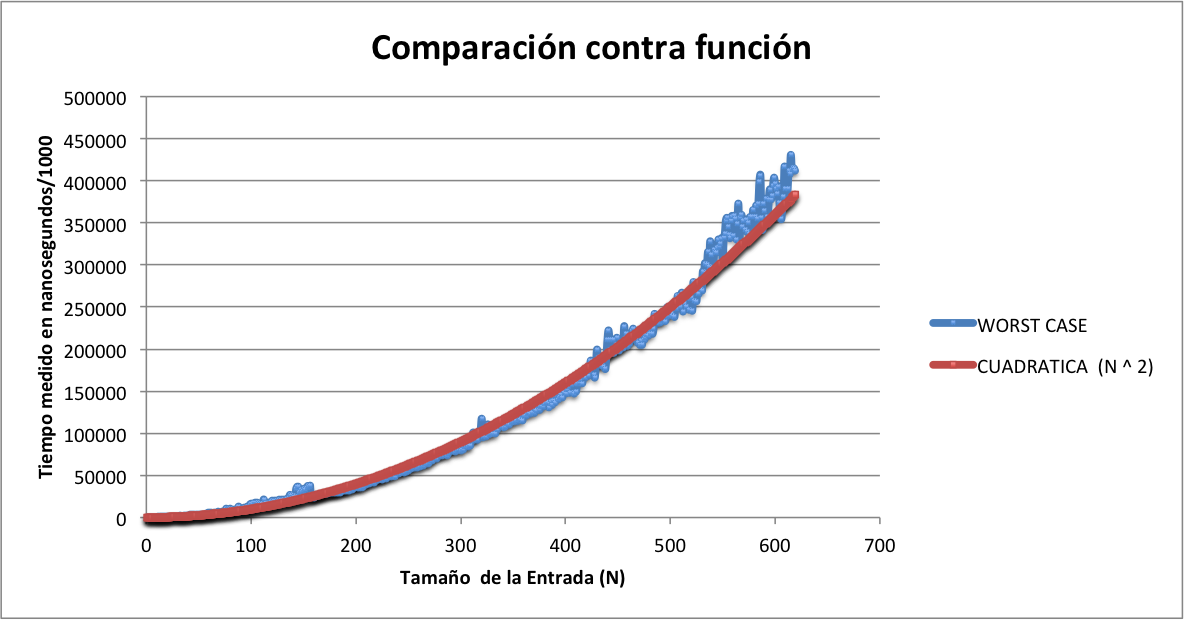
\includegraphics[width=120mm]{ej2_casos.png}
\centering
\caption{Peor caso en comparaci\'on con una funci\'on cuadr\'atica.}
\label{overflow3}
\end{figure}
Como mencionamos antes, el peor caso sucede cuando debemos recorrer todos los nodos. La cantidad de nodos viene dada por $N*L$. Para hacer los tests, decidimos utilizar edificios de forma cuadrada, es decir que la cantidad de pisos es igual a la longitud de cada piso. Para estos casos, tenemos que $L = N$. Y como se ve en el grafico, el peor caso se comporta muy similar a esta manera. 

\begin{figure}[h!]
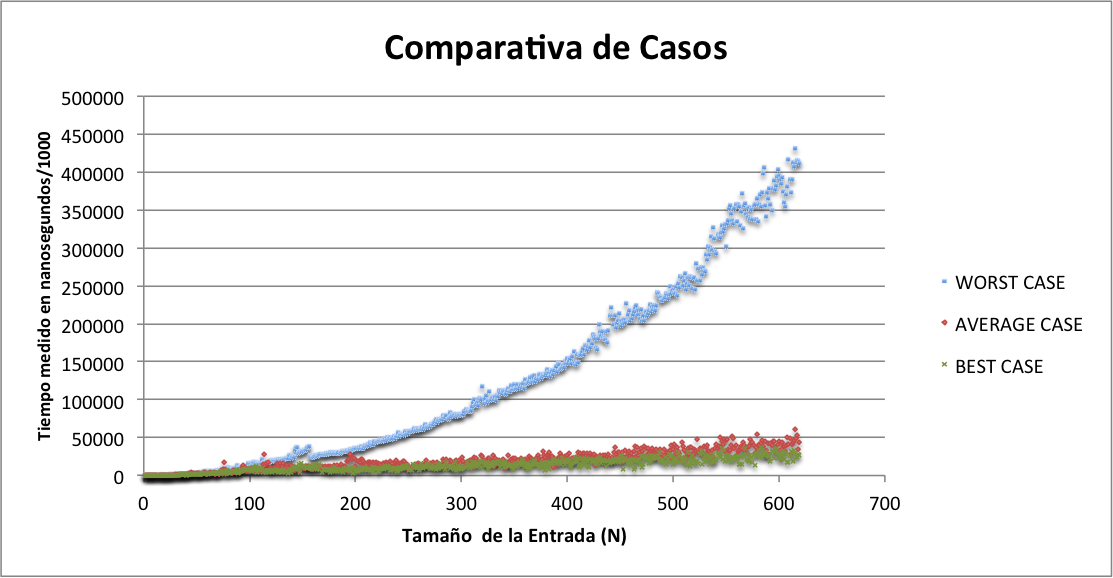
\includegraphics[width=120mm]{ej2_comp.png}
\centering
\caption{Comparaci\'on de los peores y mejores casos contra casos promedio.}
\label{overflow3}
\end{figure}
Como podemos apreciar en el grafico, el caso promedio se aleja muchisimo del peor caso ya que al general de manera pseudo-aleatoria las conexiones entre los portales, la probabilidad de tener que recorrerlos absolutamente todos ( $N*P+L$) es muy baja. Llamativamente, el caso promedio se asemeja al mejor caso. Creemos que la causa es que como un portal puede tener muchos vecinos, podemos encontrar el camino al final de manera mas rapida.

\subsubsection{Optimizado vs no optimizado}
Para mejorar el rendimiento del algoritmo se agrego una optimizacion donde al momento de encontrar el nodo buscado finalizara, a continuacion se haran algunas pruebas sobre el beneficio que brinda dicha optimizacion en los casos vistos en la secci\'on $2.4$.
\\
Primero veamos un poco el algoritmo:

\begin{lstlisting}
solve(Nodo nodo, Nodo nodo2, int i) 
	cola <- new LinkedList<Nodo>()
	cola.addFirst(nodo)
	nodo.setVisitado()
	WHILE ! cola.isEmpty()
        Nodo actual;
        actual = cola.pop()
        List<Nodo> vecinos = actual.getVecinos();		
        FOREACH vecinos AS vecino
            IF !vecino.getVisitado()
                vecino.setVisitado()
                vecino.setLongitud(actual.getLongitud()+1)
			cola.push(vecino)
	        ENDIF
     	ENDFOR
    ENDWHILE
DEVOLVER nodo2.getLongitud()
\end{lstlisting}

Por como esta dado simplemente chequeara todos los nodos y, al terminar, quedara en $nodo2$ la longitud minima, a continuacion se considerara el siguiente codigo:

\begin{lstlisting}
solve(Nodo nodo, Nodo nodo2, int i) 
	cola <- new LinkedList<Nodo>()
	cola.addFirst(nodo)
	nodo.setVisitado()
	encontrado <- false
	WHILE !cola.isEmpty() AND !encontrado
        Nodo actual;
        actual = cola.pop()
        List<Nodo> vecinos = actual.getVecinos();		
        FOR i<-0 WHILE i<vecinos.size() AND !encontrado STEP i++ 
            vecino <- vecinos.obtener(i)
            IF !vecino.getVisitado()
                vecino.setVisitado()
                vecino.setLongitud(actual.getLongitud()+1)
                IF actual.getId() == nodo2.getId()
                    encontrado <- true
                ENDIF
            cola.push(vecino)
            ENDIF
     	ENDFOR
    ENDWHILE
DEVOLVER nodo2.getLongitud()
\end{lstlisting}

La variable encontrado sera colocada en true al momento de toparse con el nodo que era buscado, a primera vista esto deberia mejorar la performance del algoritmo, para ello se hara un analisis de cada caso: \\\\

\begin{centering}
Peor Caso \\
\end{centering}

\begin{figure}[h!]
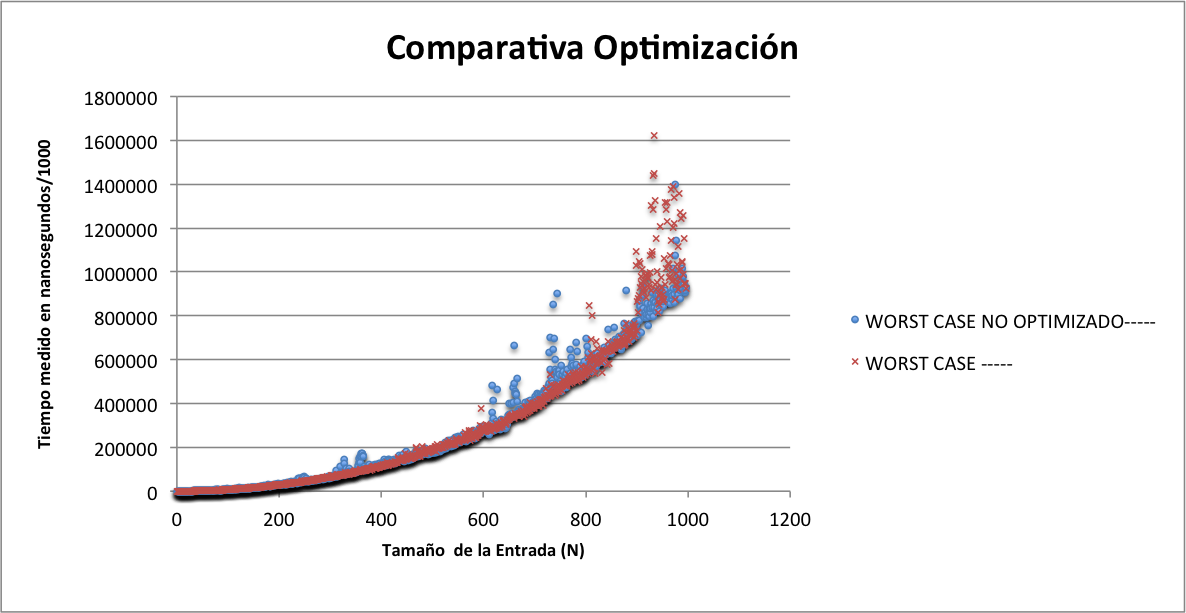
\includegraphics[width=140mm]{ej2-comp-tp2.png}
\centering
\caption{Comparacion peores casos}
\label{overflow3}
\end{figure}

En la imagen se puede observar que no hay una gran diferencia entre los dos algoritmos, esto se debe a que en el peor caso solo habra una conexion con el ultimo piso y esta estara al final del recorrido, por lo que cualquiera de los dos algoritmos debera recorrer todo el grafo hasta llegar al nodo buscado. Incluso podemos decir que el algoritmo optimizado puede tardar un poco ya que posee $3$ chequeos intermedios sobre la variable $encontrado$, que si bien no es un gran cambio afecta un poco.\\\\

\pagebreak

\begin{centering}
Mejor Caso \\
\end{centering}

\begin{figure}[h!]
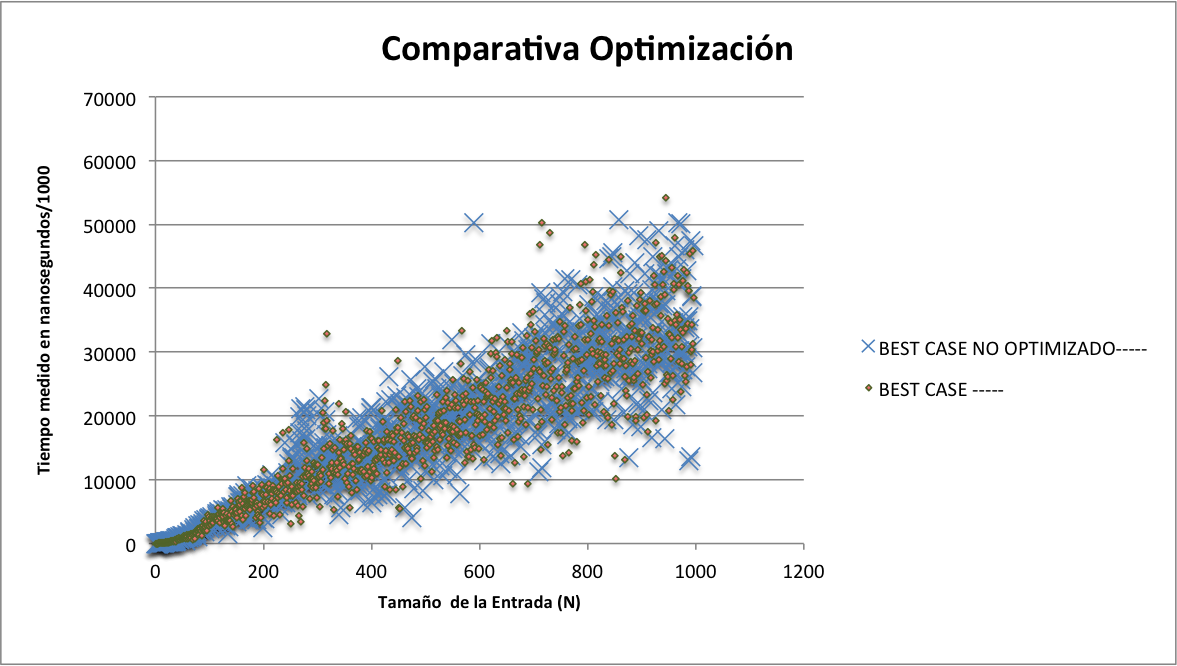
\includegraphics[width=140mm]{ej2-comp2-tp2.png}
\centering
\caption{Comparacion mejores casos}
\label{overflow3}
\end{figure}

En el mejor caso se construyo el grafo de manera que hubiera un portal apenas comienza el piso $0$ que conecte con el final del ultimo piso. Se espero que el rendimiento del algoritmo optimizado fuera superior al otro pero en el grafico se puede observar que no. 

\begin{figure}[h!]
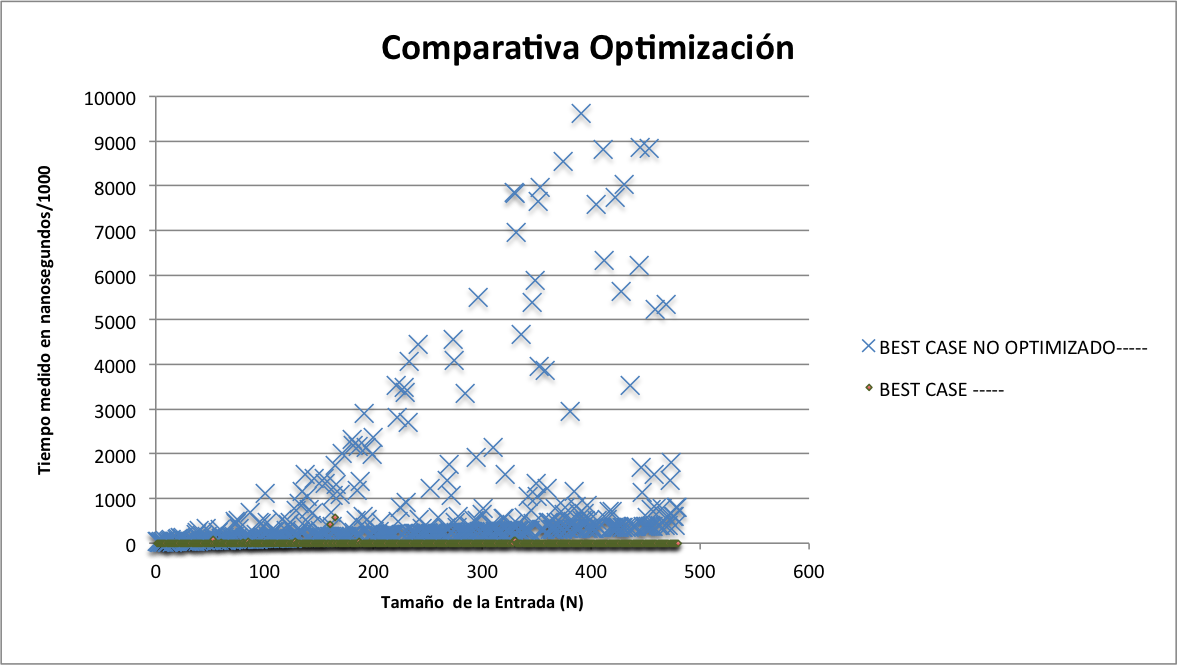
\includegraphics[width=140mm]{ej2-compesp-tp2.png}
\centering
\caption{Comparacion cantidad de iteraciones mejores casos}
\label{overflow3}
\end{figure}

Haciendo mas pruebas se pudo ver que el algoritmo optimizado casi siempre hizo $4$ iteraciones (ya que al tener portales lanzados aleatoriamente puede haberlo enviado a otro lugar) antes de terminar mientras que el otro tuvo cantidad variable y creciente, lo que contradice el primer grafico. La hipotesis es que hay algun costo externo que no pudo ser observado en la experimentacion. Pero teoricamente y por la prueba de iteraciones maximas podemos decir que el algoritmo optimizado para este caso es mucho mas efectivo que el otro, teniendo un costo de $4$ iteraciones constantemente.\\\\

\pagebreak

\begin{centering}
Caso General \\
\end{centering}

\begin{figure}[h!]

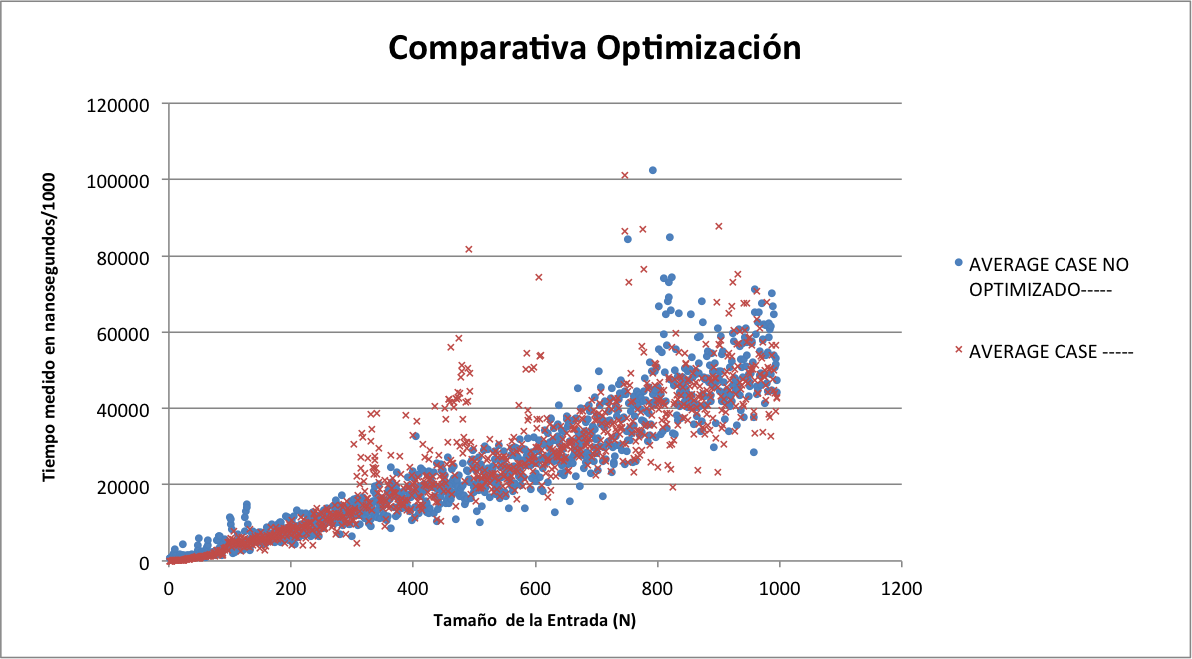
\includegraphics[width=140mm]{ej2-comp1-tp2.png}
\centering
\caption{Comparacion casos generales}
\label{overflow3}
\end{figure}

En el caso general el algoritmo optimizado tuvo un poco mas de rendimiento que el otro, se puede observar en el grafico que su curva tiene una pendiente menos eleveda que el no optimizado, como en el caso general no sabemos cual es el camino general, el primer algoritmo tiende a ser un poco mejor.


\pagebreak
Luego decidimos comparar el mejor y peor caso del algoritmo, y analizamos los tiempos teniendo en cuenta la creaci\'on del grafo o no. En la siguiente imagen se observa la gran diferencia de tiempos y esto es debido al gran costo de incializaci\'on de estructuras.
\begin{figure}[h!]
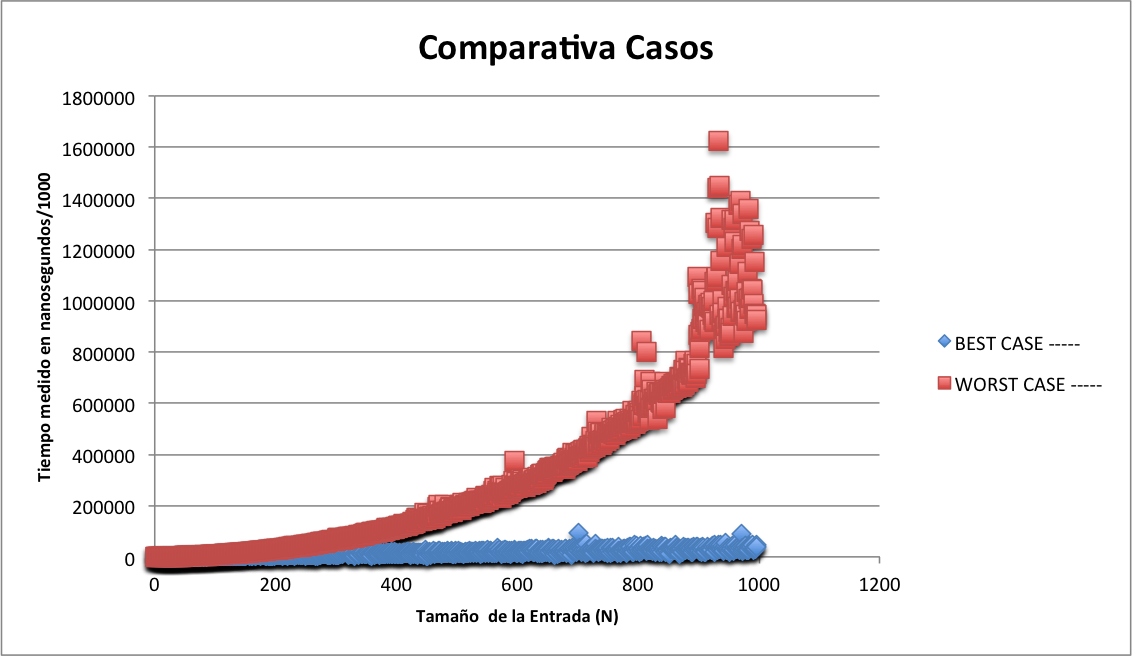
\includegraphics[width=140mm]{ej2-compcasos-tp2.png}
\centering
\caption{Comparacion Best Vs Worst}
\label{overflow3}
\end{figure}

\pagebreak

